\section{Design 2} \label{sec:design-log}
\begin{figure*}
    \centering
    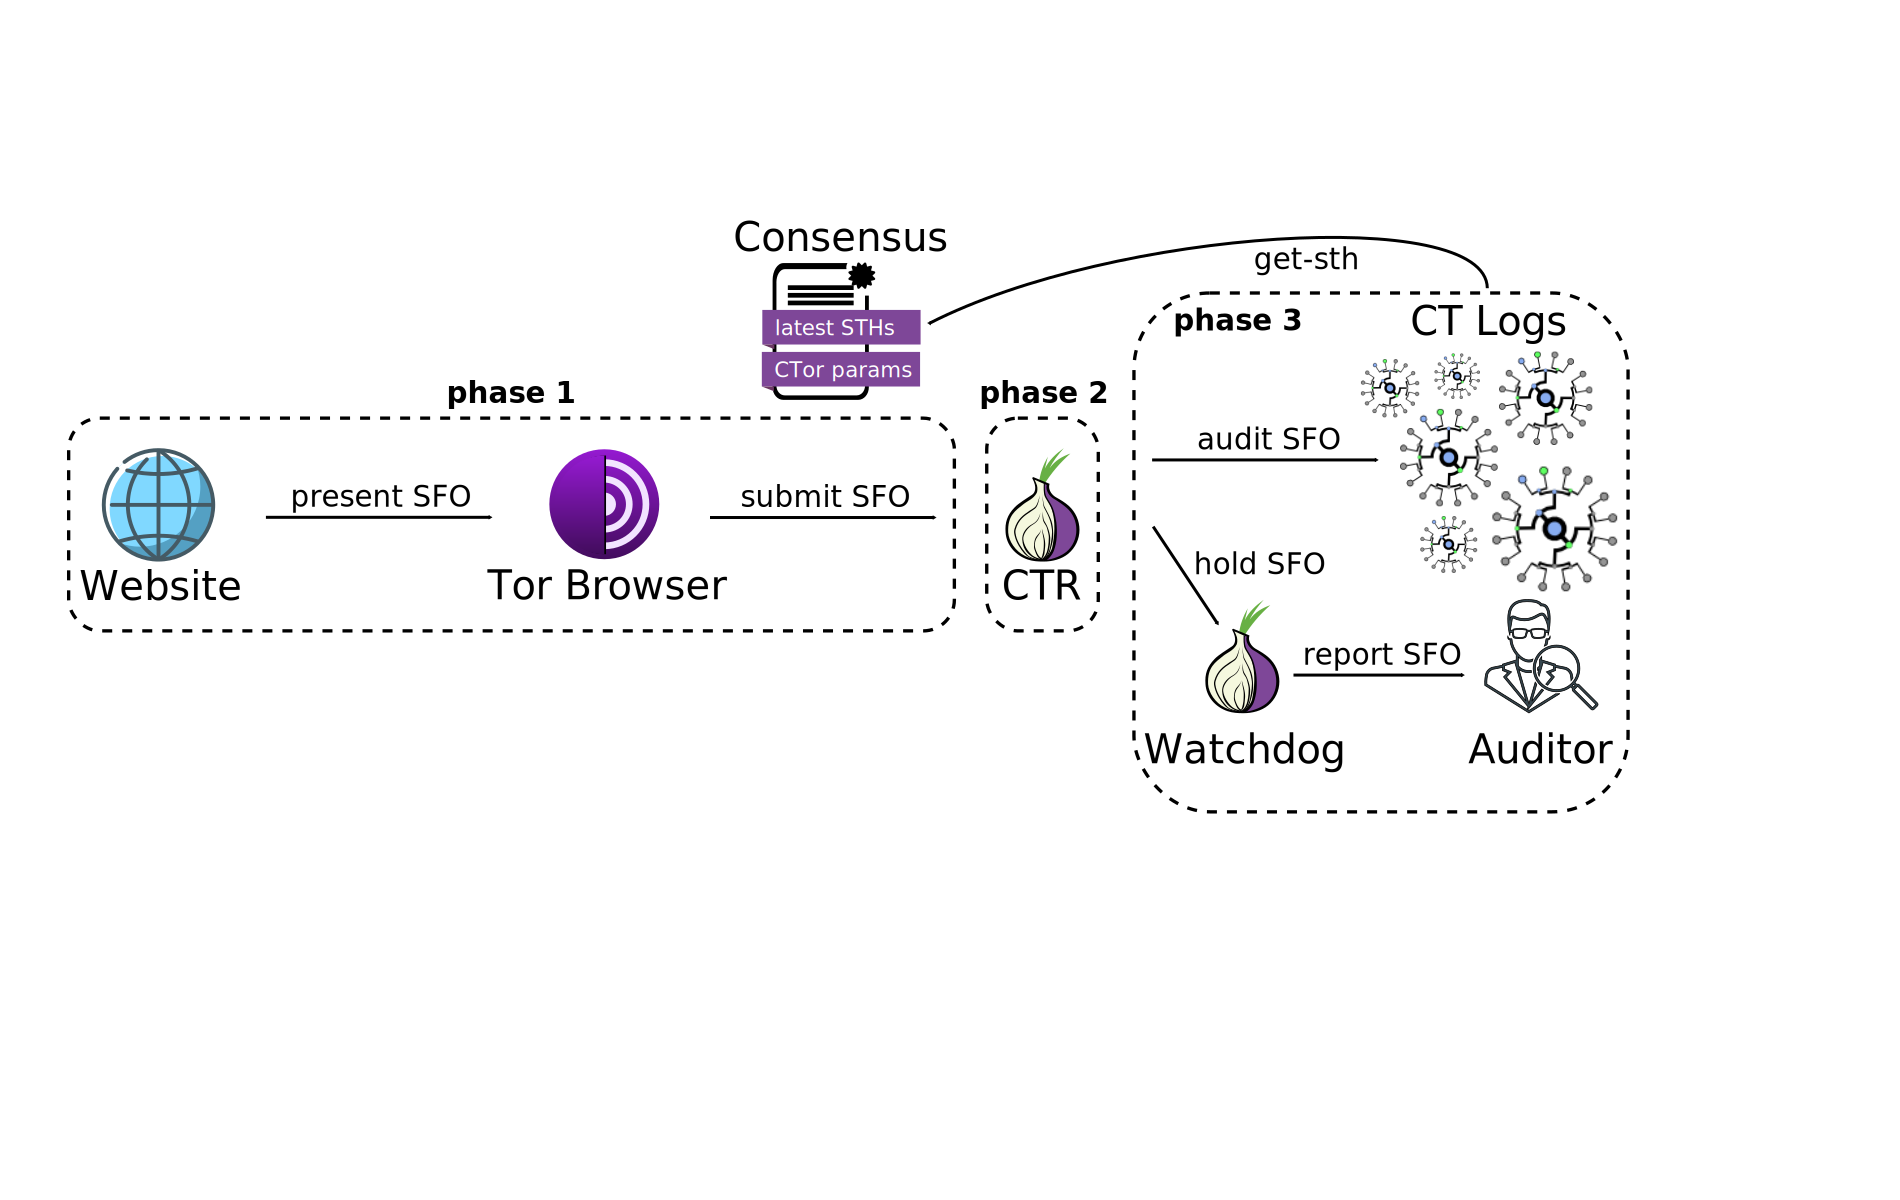
\includegraphics[width=0.85\textwidth]{img/setting-log}
    \caption{An overview of our design: Tor's consensus is extended by including
        the latest STH from each relevant CT log (periodically fetched by
        Directory Authorities) together with global CTor parameters (presented
        throughout Section~\ref{sec:design}). A website presents a SFO to Tor
        Browser, and Tor Browser in turn submits this SFO with some probability
        (consensus parameter) to a randomly selected CTR (phase 1). The CTR
        temporarily stores the SFO (phase 2). After some random delay (another
        parameter), the CTR attempts to audit the SFO by challening the issuing
        CT log using the STH in the consensus (phase 3). Upon failed audit, the
        SFO is reported to a trusted auditor listed in the consensus (phase 4).
        All connections are made over dedicated independent circuits.}
    \label{fig:overview2}
\end{figure*}